%保存为UTF-8编码格式
%用xelatex编译
 
\documentclass[UTF8,a4paper,12pt]{ctexart}
\usepackage[left=2.50cm, right=2.50cm, top=2.50cm, bottom=2.50cm]{geometry} %页边距
\CTEXsetup[format={\Large\bfseries}]{section} %设置章标题字号为Large,居左
%\CTEXsetup[number={\chinese{section}}]{section}
%\CTEXsetup[name={(,)}]{subsection}
%\CTEXsetup[number={\chinese{subsection}}]{subsection}
%\CTEXsetup[name={(,)}]{subsubsection}
%\CTEXsetup[number=\arabic{subsubsection}]{subsubsection}  %以上四行为各级标题样式设置,可根据需要做修改
 
%\linespread{1.5} %设置全文行间距
 
 
%\usepackage[english]{babel}
%\usepackage{float}     %放弃美学排版图表
\usepackage{fontspec}   %修改字体
\usepackage{amsmath, amsfonts, amssymb} % 数学公式相关宏包
\usepackage{color}      % color content
\usepackage{graphicx}   % 导入图片
\usepackage{subfigure}  % 并排子图
\usepackage{url}        % 超链接
\usepackage{bm}         % 加粗部分公式,比如\bm{aaa}aaa
\usepackage{multirow}
\usepackage{booktabs}
\usepackage{epstopdf}
\usepackage{epsfig}
\usepackage{longtable}  %长表格
\usepackage{supertabular}%跨页表格
\usepackage{algorithm}
\usepackage{algorithmic}
\usepackage{changepage}
 
 
 
%%%%%%%%%%%%%%%%%%%%%%%
% -- text font --
% compile using Xelatex
%%%%%%%%%%%%%%%%%%%%%%%
% -- 中文字体 --
%\setCJKmainfont{Microsoft YaHei}  % 微软雅黑
%\setCJKmainfont{YouYuan}  % 幼圆
%\setCJKmainfont{NSimSun}  % 新宋体
%\setCJKmainfont{KaiTi}    % 楷体
\setCJKmainfont[AutoFakeBold=true]{SimSun}   % 宋体
%\setCJKmainfont{SimHei}   % 黑体
 
% -- 英文字体 --
\setmainfont{Times New Roman}
%\setmainfont{DejaVu Sans}
%\setmainfont{Latin Modern Mono}
%\setmainfont{Consolas}
%
%
\renewcommand{\algorithmicrequire}{ \textbf{Input:}}     % use Input in the format of Algorithm
\renewcommand{\algorithmicensure}{ \textbf{Initialize:}} % use Initialize in the format of Algorithm
\renewcommand{\algorithmicreturn}{ \textbf{Output:}}     % use Output in the format of Algorithm
\renewcommand{\abstractname}{\textbf{\large {摘\quad 要}}} %更改摘要二字的样式
\newcommand{\xiaosi}{\fontsize{12pt}{\baselineskip}}     %\xiaosi代替设置12pt字号命令,不加\selectfont,行间距设置无效
\newcommand{\wuhao}{\fontsize{10.5pt}{10.5pt}\selectfont}
 
\usepackage{fancyhdr} %设置全文页眉、页脚的格式
\pagestyle{fancy}
\lhead{}           %页眉左边设为空
\chead{}           %页眉中间
\rhead{}           %页眉右边
%\rhead{\includegraphics[width=1.2cm]{1.eps}}  %页眉右侧放置logo
\lfoot{}          %页脚左边
\cfoot{\thepage}  %页脚中间
\rfoot{}          %页脚右边
 
 
%%%%%%%%%%%%%%%%%%%%%%%
%  设置水印
%%%%%%%%%%%%%%%%%%%%%%%
%\usepackage{draftwatermark}         % 所有页加水印
%\usepackage[firstpage]{draftwatermark} % 只有第一页加水印
% \SetWatermarkText{Water-Mark}           % 设置水印内容
% \SetWatermarkText{\includegraphics{fig/ZJDX-WaterMark.eps}}         % 设置水印logo
% \SetWatermarkLightness{0.9}             % 设置水印透明度 0-1
% \SetWatermarkScale{1}                   % 设置水印大小 0-1
 
\usepackage{hyperref} %bookmarks
\hypersetup{colorlinks, bookmarks, unicode} %unicode
 
 
 
\title{\textbf{\Large{中文报告\LaTeX{}模板}}}
\author{ Author\thanks{footnotes} }
%\date{\today}
%\date{2021/10/21}
 
 
 
\begin{document}
 
\maketitle
%\tableofcontents
 
% \begin{abstract}
% 本模板可以提供一般性单栏文档的生成,可以根据需要选择是否要目录、摘要,可自行选择日期生成方式,参考文献使用交叉引用条目形式使用,便于编辑和管理。务必注意,latex编译器需要选择xelatex.
% \end{abstract}
 
% \begin{center}
% \large{\textbf{Abstract}}
% \end{center}
 
\begin{adjustwidth}{1cm}{1cm}
\hspace{1.5em}Here is the first par. of abstract.Here is the first par. of abstract.
 
\noindent\hspace{1.5em}Here is the second par. of abstract.Here is the second par. of abstract.
\end{adjustwidth}
 
%\thispagestyle{empty}       %本页不显示页码
%\newpage                    %分页
%%\tableofcontents\thispagestyle{empty}
%\newpage
%\setcounter{page}{1}        %从下面开始编页,页脚格式为导言部分设置的格式
 
 
\section{第一部分}
这是第一部分
\subsection{第一部分的子部分}
这里是第一部分的子部分
 
\section{第二部分}
这里是第二部分 \cite{ref1,ref2}
\subsection{第二部分的子部分}
这里是第二部分的子部分
 
\section{一些工具}
插入公式
\begin{equation}\label{eq}
  \gamma _2^{\text{C}} = \frac{{{P_{RT}}g}}{{{P_{BT}}d_{_{{B_2}2}}^{ - \alpha } + {N_0}}}
\end{equation}
 
%插入图片
%\begin{figure}[H]   %*表示可跨栏,如果不需要可去掉
%\centering
%\subfigure[$\sum {{I_C}}  < {I_B}$]{
%  \includegraphics[width=7cm]{1.eps}}
%  %\hspace{0cm}      %两张图片之间的距离
%%\hfill               %撑满整行
%\centering
%\subfigure[$\sum {{I_C}}  > {I_B}$]{
%  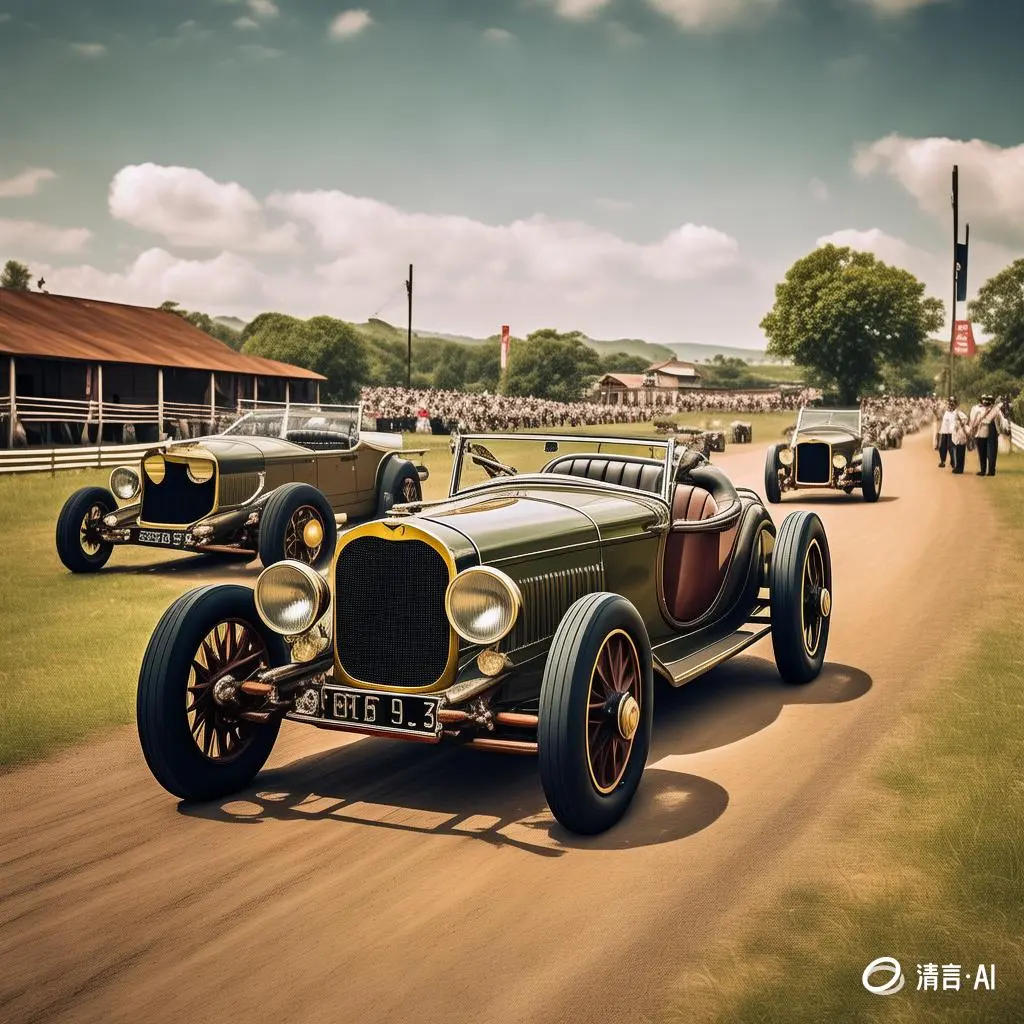
\includegraphics[width=7cm]{2.eps}}
%\caption{系统的模式选择}\label{fig}
%\end{figure}
 
插入表格
\begin{table}[H] \wuhao             %局部字体设置大小
   \centering
  \caption{系统模型符号}\label{tab}
  \begin{tabular}{c|c}
    \toprule                  %设置为顶线默认格式 加粗
    % after \\: \hline or \cline{col1-col2} \cline{col3-col4} ...
    符号 & 说明 \\
    \hline                  %普通横线
    ${{B_1}\mbox{、}{B_2}}$ & 基站的下标表示 \\
    ${C_1}\mbox{、}{C_2}$ & 蜂窝用户的下标表示 \\
    $D$ & D2D用户的下标表示 \\
    $R$ & 中继用户的下标表示 \\
    ${P_{it}}\left( {i = B,C,D,R} \right)$ & 终端$i$的发射功率 \\
    ${d_{ij}}(i,j = {B_k},{C_k},1,2,R;i \ne j,k = 1,2)$ & 设备$i$到设备$j$的距离 \\
    ${h_{ij}}(i,j = {B_k},{C_k},1,2,R;i \ne j,k = 1,2)$ &$i$-$j$ 链路的信道系数\\
    ${n_i}\left( {{n_i}\sim N\left( {\mu ,{N_0}} \right)} \right)$ & 高斯白噪声 \\
    ${P_{ij}} = {P_{iT}}d_{ij}^{ - \alpha }$ & 终端$j$收到的终端$i$发送的信号功率\\
    $\alpha$ & 路径衰落系数 \\
    \bottomrule                %设置为底线默认格式
  \end{tabular}
\end{table}
 
%引用:图\ref{fig},式\eqref{eq},表\ref{tab}

\begin{thebibliography}{99}
	\setlength{\parskip}{0pt} %段落之间的竖直距离
	\bibitem{ref1}吴承恩. 西游记~[M], 明14XX年.
	\bibitem{ref2} 玄奘. 大唐西域记学报~[J], 唐6XX年, 1(2): 23-55.
\end{thebibliography}

\end{document}

